\documentclass[12pt]{article}
\usepackage[utf8]{inputenc}
\usepackage{indentfirst}
\usepackage{pdfpages}
\usepackage{graphicx}
\usepackage{hyperref}
\hypersetup{
    colorlinks,
    citecolor=black,
    filecolor=black,
    linkcolor=red,
    urlcolor=black,
}

\title{\textbf{PyTorch Lightning}}
\author{Maxime Cheniour \\ Octave Cinquanta}
\date{March 2023}

\begin{document}

\maketitle

\tableofcontents


\section{Introduction}

\subsection{A Brief Description of PyTorch Lightning}

PyTorch Lightning is a high-level, open-source deep learning framework built on top of PyTorch.
It was developed to simplify the training, validation, and testing processes of deep learning models while retaining the flexibility and performance of the PyTorch framework.
By providing a structured, standardized approach to deep learning model development, PyTorch Lightning aims to reduce the complexity and boilerplate code that is often associated with PyTorch.

One of the primary goals of PyTorch Lightning is to enable researchers and practitioners to focus on the core ideas and algorithms behind their models, rather than spending time on low-level implementation details.
It achieves this by abstracting away much of the boilerplate code, such as managing data loading, model optimization, and distributed training, into a set of modular, reusable components.
These components include LightningModule, LightningDataModule, Trainer, and various callbacks and loggers.

By adopting PyTorch Lightning, users can easily scale their models across multiple GPUs, TPU cores, or even clusters, without changing the core model code.
The framework also promotes best practices in deep learning, such as code organization, reproducibility, and modularity, which can lead to more efficient and maintainable projects.
Additionally, PyTorch Lightning offers seamless integration with popular tools and services in the machine learning ecosystem, such as TensorBoard, Weights \& Biases, and Neptune.ai, facilitating experiment tracking, visualization, and collaboration.

\subsection{Purpose of the Report}

The purpose of this report is to provide a comprehensive overview and analysis of the PyTorch Lightning framework, highlighting its key components, benefits, and limitations.
It aims to equip the readers with a better understanding of PyTorch Lightning's features and functionality, enabling them to make informed decisions when choosing a deep learning framework for their projects.

Additionally, the report will draw comparisons between PyTorch Lightning and other popular deep learning frameworks to help readers gain insights into the unique strengths and weaknesses of each.
By presenting use cases and applications of PyTorch Lightning in various domains, the report seeks to demonstrate the framework's versatility and potential impact on the development of deep learning models.

Lastly, this report will outline best practices and tips for using PyTorch Lightning effectively and efficiently, as well as explore the future developments and trends in the framework.
By doing so, the report aims to contribute to the growth and adoption of PyTorch Lightning within the deep learning community.

\section{Background}

\subsection{A PyTorch Framework}

\subsubsection{Overview}

PyTorch is an open-source deep learning framework developed by Facebook's AI Research Lab (FAIR). Released in 2016, it has quickly become one of the most popular tools for building and training neural networks in research and industry.
PyTorch provides a flexible, Pythonic interface that allows developers to define, train, and deploy deep learning models using dynamic computation graphs and automatic differentiation.

\subsubsection{Features and Benefits}

\begin{itemize}
    \item Dynamic Computation Graphs (Eager Execution): Unlike other deep learning frameworks, which use static computation graphs, PyTorch employs dynamic computation graphs, also known as eager execution. This approach allows for more intuitive debugging and greater flexibility when designing complex models with dynamic control flow, such as recurrent neural networks (RNNs) or models with varying input sizes.
    \item Automatic Differentiation: PyTorch's autograd package enables automatic differentiation for all operations on tensors. This feature simplifies the computation of gradients, which are crucial for optimizing neural network parameters using backpropagation.
    \item GPU Acceleration: PyTorch natively supports NVIDIA GPUs, offering seamless integration with CUDA and cuDNN libraries. This enables users to harness the power of GPU acceleration for faster model training and inference.
    \item Extensive Library and Community Support: PyTorch boasts a vast ecosystem of libraries and tools, covering various aspects of deep learning, such as computer vision (Torchvision), natural language processing (Torchtext), and reinforcement learning (TorchRL). The active community contributes to the development of new features and provides extensive support through forums, tutorials, and conferences.
    \item Interoperability: PyTorch offers excellent interoperability with other popular Python libraries, such as NumPy, Pandas, and Scikit-learn. This allows users to easily integrate PyTorch into their existing data processing and machine learning workflows.
    \item Research to Production: PyTorch supports the entire deep learning pipeline, from research and experimentation to production deployment. With tools like TorchScript and the PyTorch JIT compiler, users can optimize and export their models to production environments, including mobile and embedded devices.
\end{itemize}

\subsection{Motivation for PyTorch Lightning}

\subsubsection{Challenges in using PyTorch}

While PyTorch offers flexibility and ease of use, it also presents some challenges that can hinder the development process, especially for complex models and large-scale projects. Some of these challenges include:

\begin{itemize}
    \item Boilerplate Code: Users often need to write repetitive code for tasks such as data loading, model training, validation, and testing. This can lead to longer development times and a higher probability of errors.
    \item Lack of Standardization: PyTorch does not enforce a specific structure or organization for deep learning projects. As a result, developers may adopt different coding styles, making it difficult to share, collaborate, or maintain projects within the community.
    \item Scalability: Scaling models to multiple GPUs, TPUs, or distributed clusters can be complex and require a significant amount of additional code. This can be time-consuming and prone to errors, especially for researchers and developers who may not be familiar with parallel and distributed computing paradigms.
\end{itemize}

\subsubsection{Need for a more streamlined and standardized approach}

Given the aforementioned challenges, there is a clear need for a more streamlined and standardized approach to deep learning development using PyTorch.
PyTorch Lightning aims to address these issues by providing a high-level framework that abstracts away boilerplate code, enforces best practices, and simplifies the process of scaling models across different hardware configurations.

By adopting PyTorch Lightning, users can focus on the core ideas and algorithms behind their models, without worrying about the low-level implementation details.
The framework also encourages modularity and code reusability, making it easier to share and collaborate on projects within the deep learning community.
Overall, PyTorch Lightning seeks to make the process of developing, training, and deploying deep learning models using PyTorch more efficient, maintainable, and accessible to a wider audience.

\section{PyTorch Lightning Components}

\subsection{LightningModule}

\subsubsection{Structure and Purpose}

The LightningModule is the core component of PyTorch Lightning and serves as a container for organizing the code related to the model architecture, training, validation, and testing.
It is a subclass of the PyTorch nn.Module and encapsulates all the essential elements of a deep learning model, ensuring a clean, modular, and reusable structure.

The primary purpose of the LightningModule is to simplify model development and promote best practices by separating the research code (model architecture and algorithm) from the engineering code (data loading, training loop, and distributed training).
This separation enables users to focus on the core concepts of their models while abstracting away the boilerplate code.

\subsubsection{Advantages and Features}

\begin{itemize}
    \item Organized Code Structure: The LightningModule enforces a clear organization of code, separating the model's architecture, optimization, and data handling. This structure makes it easier to understand, maintain, and share the code within the community.
    \item Plug-and-Play Components: The LightningModule allows users to define the model's components, such as the optimizer, loss function, and learning rate scheduler, as independent, reusable functions. This modularity makes it easy to experiment with different configurations and swap components as needed.
    \item Automatic Optimization: The LightningModule automatically handles the forward and backward passes, gradient calculation, and parameter updates, allowing users to focus on the model's logic instead of the optimization process.
    \item Built-in Training Loop: PyTorch Lightning provides a default training loop that handles the training, validation, and testing processes. Users can override this loop to customize it or use the built-in loop for a streamlined, hassle-free implementation.
    \item Device-Agnostic: The LightningModule is designed to be device-agnostic, meaning it can seamlessly run on CPUs, GPUs, or TPUs without requiring any changes to the model code.
    \item Automatic Mixed Precision (AMP) and Distributed Training: The LightningModule supports automatic mixed precision training and distributed training, allowing users to scale their models across multiple GPUs, TPU cores, or even clusters with minimal code changes.
\end{itemize}

\subsection{LightningDataModule}

\subsubsection{Structure and Purpose}

The LightningDataModule is another key component of PyTorch Lightning, designed to manage and decouple data-related aspects of a deep learning project.
It is a flexible and reusable class that encapsulates all data handling processes, such as data loading, preprocessing, splitting, and augmentation.

The primary purpose of the LightningDataModule is to provide a clean and organized way to handle data, making it easier to share and reuse data processing code across different projects.
By abstracting away data-related tasks from the LightningModule, it allows users to focus on the model architecture and training logic, while ensuring that the data pipeline remains consistent and maintainable.

\subsubsection{Advantages and Features}

\begin{itemize}
    \item Data Preprocessing and Augmentation: The LightningDataModule provides a structured way to define and apply data preprocessing and augmentation techniques. By encapsulating these operations within the data module, users can easily experiment with different preprocessing strategies without affecting the model code.
    \item Train-Validation-Test Split: The LightningDataModule offers built-in support for splitting the dataset into training, validation, and test sets. This ensures a consistent and reproducible data pipeline across different experiments.
    \item Custom Data Loaders: Users can define custom data loaders in the LightningDataModule, allowing for greater flexibility when working with different data formats and sources. This makes it easier to adapt the data pipeline to specific project requirements.
    \item Scalability: The LightningDataModule supports scalable data loading, which is essential when working with large datasets or distributed training. It automatically handles data loading across multiple GPUs, TPUs, or nodes, ensuring that the data pipeline scales efficiently with the model.
    \item Reusability and Shareability: By encapsulating data handling in the LightningDataModule, users can create reusable and shareable data pipelines. This promotes collaboration and code reusability within the deep learning community, as well as making it easier to switch between different datasets or tasks.
    \item Clean Separation of Concerns: The LightningDataModule promotes a clean separation of concerns between data handling and model development. This separation simplifies the overall project structure, making it more maintainable and easier to understand.
\end{itemize}

\subsection{Trainer}

\subsubsection{Structure and Purpose}

The Trainer is a central component in PyTorch Lightning that manages the training, validation, and testing processes.
It is a high-level class that automates the training loop and provides a range of features and utilities to simplify model training and evaluation.

The primary purpose of the Trainer is to allow users to focus on the research aspects of their models, such as architecture and algorithm design, while abstracting away the engineering complexities of the training loop, optimization, and hardware management.
By providing a range of pre-built features and utilities, the Trainer streamlines the model training process, making it more accessible and efficient.

\subsubsection{Advantages and Features}

\begin{itemize}
    \item Automated Training Loop: The Trainer automates the training loop, handling epoch and batch iteration, model optimization, and evaluation metrics. This reduces the amount of boilerplate code required, allowing users to focus on the core logic of their models.
    \item Configurable Callbacks: The Trainer supports a range of built-in and custom callbacks that can be used to add functionality during the training process. Callbacks enable users to implement features such as model checkpointing, early stopping, and learning rate scheduling with minimal effort.
    \item Mixed Precision and Distributed Training: The Trainer provides built-in support for automatic mixed precision (AMP) and distributed training, allowing users to scale their models across multiple GPUs, TPU cores, or clusters with minimal code changes.
    \item Logging and Visualization: The Trainer offers seamless integration with popular logging and visualization tools, such as TensorBoard, Weights \& Biases, and Neptune.ai. This facilitates experiment tracking, model evaluation, and collaboration among team members.
    \item Device-Agnostic: The Trainer is designed to be device-agnostic, ensuring that models can run on CPUs, GPUs, or TPUs without any changes to the code.
    \item Customizability: The Trainer provides a range of configuration options and hooks that allow users to customize the training process to suit their specific needs. This flexibility makes it easy to adapt the Trainer to different project requirements and constraints.
\end{itemize}

\subsection{Callbacks and Loggers}

\subsubsection{Overview}

Callbacks and loggers are essential components in PyTorch Lightning that enable users to extend and customize the functionality of the training process.
They provide a mechanism to perform specific actions at different stages of the training loop, such as modifying model behavior, logging metrics, or changing learning rates.

\subsubsection{Pre-built and Custom Callbacks}

\begin{itemize}
    \item Pre-built Callbacks: PyTorch Lightning includes a variety of pre-built callbacks that cover common use cases and can be easily integrated into the training process. Some of the popular pre-built callbacks are:
    - ModelCheckpoint: Automatically saves the model weights at specified intervals or when a particular performance metric improves. \newline
    - EarlyStopping: Stops the training process when a specified performance metric stops improving for a given number of epochs, preventing overfitting. \newline
    - LearningRateMonitor: Logs the learning rate during the training process, allowing users to visualize and analyze the learning rate schedule. \newline
    - GradientAccumulationScheduler: Accumulates gradients over a specified number of batches, effectively increasing the effective batch size without increasing memory requirements.
    \item Custom Callbacks: In addition to the pre-built callbacks, PyTorch Lightning allows users to create custom callbacks by subclassing the Callback class and implementing the desired behavior.
    Custom callbacks offer a flexible way to implement project-specific functionality or experiment with novel techniques during the training process.
\end{itemize}

\subsubsection{Logging Options and Integrations}

PyTorch Lightning's logger functionality enables users to track and visualize training metrics, hyperparameters, and model performance throughout the training process. The framework supports various popular logging tools and services, making it easy to integrate with existing workflows and tools. Some of the supported loggers include:

\begin{itemize}
    \item TensorBoard: PyTorch Lightning includes built-in support for logging to TensorBoard, Google's widely-used visualization tool for deep learning.
    \item Weights \& Biases: Integration with Weights \& Biases allows users to track and visualize experiments in real-time, compare runs, and collaborate with team members using the Weights \& Biases platform.
    \item Neptune.ai: Users can log and visualize experiments using Neptune.ai, a cloud-based experiment tracking and collaboration platform.
    \item Custom Loggers: PyTorch Lightning also supports custom loggers, allowing users to create their own logging solutions or integrate with other logging platforms as needed.
\end{itemize}

By providing a wide range of built-in callbacks and loggers, as well as support for custom implementations, PyTorch Lightning offers a highly flexible and extensible framework that can adapt to various project requirements and deep learning workflows.

\section{Comparison to Other Deep Learning Frameworks}

\subsection{TensorFlow and Keras}

\subsubsection{Overview}

TensorFlow is an open-source deep learning framework developed by Google that has gained widespread popularity for its flexibility, performance, and extensive feature set. Keras, initially an independent high-level API, was later integrated with TensorFlow and now serves as its official high-level API for building and training neural networks.

\subsubsection{Comparison with PyTorch Lightning}

\begin{itemize}
    \item Computation Graphs: TensorFlow uses static computation graphs, while PyTorch Lightning, built on top of PyTorch, employs dynamic computation graphs (eager execution). Dynamic computation graphs offer more flexibility and easier debugging, especially for models with complex control flow or varying input sizes.
    \item High-level API: Keras provides a high-level API similar to PyTorch Lightning, abstracting away boilerplate code and simplifying the model development process. However, PyTorch Lightning offers a more Pythonic approach, making it more intuitive for Python developers.
    \item Modularity: Both Keras and PyTorch Lightning promote modularity and code reusability. While Keras provides pre-built layers and models for various deep learning tasks, PyTorch Lightning enforces a clean organization of code using LightningModule and LightningDataModule.
    \item Customizability: TensorFlow and Keras offer a high degree of customizability, allowing users to create custom layers, models, and training loops. However, PyTorch Lightning's dynamic computation graph and its focus on modularity may make it easier for users to experiment with and modify their models.
    \item Scalability: TensorFlow natively supports distributed training across multiple GPUs, TPUs, and clusters. PyTorch Lightning also provides distributed training support through the Trainer component, allowing users to scale their models efficiently across different hardware configurations.
    \item Community and Ecosystem: Both TensorFlow and PyTorch Lightning boast extensive ecosystems, with numerous libraries and tools for various deep learning tasks. TensorFlow has a larger user base and more mature ecosystem, but PyTorch and PyTorch Lightning have been rapidly gaining popularity and community support.
\end{itemize}

\subsection{Fast.ai}

\subsubsection{Overview}

Fast.ai is a high-level deep learning library built on top of PyTorch that aims to make deep learning more accessible to a broader audience. The library provides a user-friendly interface for training models, with built-in best practices and an extensive collection of pre-trained models for various tasks. Fast.ai emphasizes simplicity and ease of use, enabling users to train models with minimal code and effort.

\subsubsection{Comparison with PyTorch Lightning}

\begin{itemize}
    \item Focus on Simplicity: Fast.ai prioritizes simplicity and ease of use, providing a high-level API that abstracts away many of the complexities associated with deep learning. In contrast, PyTorch Lightning focuses on flexibility and modularity, allowing users to customize their models and training processes more extensively.
    \item High-level API: Both Fast.ai and PyTorch Lightning provide high-level APIs that simplify the model development process. While Fast.ai's API is more geared towards rapid prototyping and experimentation, PyTorch Lightning's API enforces a clean organization of code through components like LightningModule and LightningDataModule.
    \item Pre-trained Models and Transfer Learning: Fast.ai offers a vast collection of pre-trained models for various tasks, making it easier for users to leverage transfer learning and quickly develop high-performance models. PyTorch Lightning, on the other hand, does not come with built-in pre-trained models but offers seamless integration with popular PyTorch model repositories, such as Torchvision and Hugging Face Transformers.
    \item Customizability: While Fast.ai allows for customization through callbacks and custom layers, PyTorch Lightning offers a higher degree of customizability and control over the model development process. The dynamic computation graph in PyTorch Lightning and its modular structure enable users to experiment with and modify their models more easily.
    \item Scalability: Both Fast.ai and PyTorch Lightning support distributed training across multiple GPUs, TPUs, and clusters. However, PyTorch Lightning provides more advanced features for distributed training, such as automatic mixed precision (AMP) and gradient accumulation.
    \item Community and Ecosystem: Fast.ai has an active community and offers comprehensive learning resources, such as online courses and tutorials, to help users get started with deep learning. PyTorch Lightning also has a growing community and is part of the larger PyTorch ecosystem, which offers extensive libraries and tools for various deep learning tasks.
\end{itemize}

\subsection{MXNet}

\subsubsection{Overview}

MXNet is an open-source deep learning framework developed by Apache that supports a wide range of programming languages, including Python, C++, and Java. It is designed for high performance, scalability, and flexibility, enabling users to develop and deploy deep learning models efficiently across various platforms and devices.

\subsubsection{Comparison with PyTorch Lightning}

\begin{itemize}
    \item Computation Graphs: MXNet supports both static and dynamic computation graphs, offering flexibility to users depending on their preferences and requirements. PyTorch Lightning, built on top of PyTorch, uses dynamic computation graphs (eager execution), which provide more flexibility and ease of debugging for models with complex control flow or varying input sizes.
    \item High-level API: MXNet provides a high-level API called Gluon, which simplifies the model development process by abstracting away low-level details. PyTorch Lightning also offers a high-level API, focusing on clean organization of code through components like LightningModule and LightningDataModule.
    \item Modularity: Both MXNet's Gluon API and PyTorch Lightning promote modularity and code reusability. While Gluon provides pre-built layers and models for various deep learning tasks, PyTorch Lightning enforces a clean organization of code using LightningModule and LightningDataModule.
    \item Customizability: MXNet and PyTorch Lightning both offer a high degree of customizability, allowing users to create custom layers, models, and training loops. However, PyTorch Lightning's dynamic computation graph and its focus on modularity may make it easier for users to experiment with and modify their models.
    \item Scalability: MXNet natively supports distributed training across multiple GPUs and clusters. PyTorch Lightning also provides distributed training support through the Trainer component, allowing users to scale their models efficiently across different hardware configurations.
    \item Community and Ecosystem: MXNet has a relatively smaller community and ecosystem compared to PyTorch and PyTorch Lightning. However, it offers extensive documentation and tutorials to help users get started with the framework.
\end{itemize}

\subsection{Criteria for Comparison}

To effectively compare PyTorch Lightning with other deep learning frameworks and libraries, such as TensorFlow and Keras, Fast.ai, and MXNet, the following criteria should be considered:

\begin{itemize}
    \item Computation Graphs: The type of computation graph (static or dynamic) supported by each framework can impact flexibility, ease of debugging, and adaptability to varying input sizes and complex control flows.
    \item High-level API: The availability of a high-level API simplifies model development and training, enabling users to focus on research aspects rather than low-level implementation details.
    \item Modularity and Code Organization: A clean organization of code using modular components enhances reusability, maintainability, and collaboration.
    \item Customizability: The ability to create custom layers, models, and training loops allows users to adapt the framework to specific project requirements and experiment with novel techniques.
    \item Scalability: Efficient distributed training support across multiple GPUs, TPUs, or clusters ensures that models can be scaled to handle large datasets and complex architectures.
    \item Pre-trained Models and Transfer Learning: Access to pre-trained models and transfer learning capabilities can significantly speed up model development and improve performance, especially for users with limited computational resources.
    \item Logging and Visualization: Integration with popular logging and visualization tools, such as TensorBoard and Weights \& Biases, simplifies experiment tracking, model evaluation, and collaboration.
    \item Callbacks and Extensibility: The availability of built-in callbacks and the ability to create custom callbacks enables users to extend and customize the functionality of the training process.
    \item Community and Ecosystem: A strong community and ecosystem contribute to the availability of learning resources, libraries, and tools that can help users get started with the framework and develop models more efficiently.
\end{itemize}

\section{Use Cases and Applications}

\subsection{Computer Vision}

\subsubsection{Overview}

Computer vision is a subfield of artificial intelligence focused on enabling computers to understand, interpret, and process visual data from the world. Deep learning has become an essential technique for solving a wide range of computer vision tasks, such as image classification, object detection, semantic segmentation, and image generation.

\subsubsection{PyTorch Lightning in Computer Vision}

PyTorch Lightning is well-suited for computer vision tasks due to its flexibility, modularity, and extensive features. By using PyTorch Lightning, users can develop and train computer vision models efficiently while leveraging the following benefits:

\begin{itemize}
    \item Modular Design: PyTorch Lightning's modular design, encompassing LightningModule and LightningDataModule, allows users to separate the model architecture and data processing logic, resulting in cleaner and more reusable code.
    \item Customizability: The flexibility of PyTorch Lightning enables users to easily create custom layers, models, and training loops, allowing for the development of novel architectures and techniques specific to computer vision tasks.
    \item Distributed Training: PyTorch Lightning's Trainer component provides built-in support for distributed training across multiple GPUs, TPUs, and clusters, making it easier to scale computer vision models for large datasets and complex architectures.
    \item Integration with PyTorch Ecosystem: PyTorch Lightning seamlessly integrates with popular PyTorch-based computer vision libraries, such as Torchvision, Detectron2, and Segmentation Models PyTorch, giving users access to pre-trained models, advanced architectures, and data augmentation techniques specific to computer vision tasks.
    \item Callbacks and Loggers: PyTorch Lightning's built-in callbacks and loggers facilitate the tracking, visualization, and evaluation of model performance during training, which is essential for iterating and improving computer vision models.
\end{itemize}

\subsection{Natural Language Processing}

\subsubsection{Overview}

Natural language processing (NLP) is a subfield of artificial intelligence that focuses on enabling computers to understand, interpret, and generate human language. Deep learning has revolutionized NLP, leading to significant advancements in tasks such as sentiment analysis, machine translation, text summarization, and question answering.

\subsubsection{PyTorch Lightning in Natural Language Processing}

PyTorch Lightning is an excellent choice for developing and training NLP models due to its flexibility, modularity, and powerful features. Users working on NLP tasks can leverage PyTorch Lightning for the following benefits:

\begin{itemize}
    \item Modular Design: PyTorch Lightning's modular design, including LightningModule and LightningDataModule, allows users to separate the model architecture and data processing logic, leading to cleaner and more reusable code.
    \item Customizability: The flexibility of PyTorch Lightning enables users to create custom layers, models, and training loops, allowing for the development of novel architectures and techniques specific to NLP tasks.
    \item Distributed Training: PyTorch Lightning's Trainer component provides built-in support for distributed training across multiple GPUs, TPUs, and clusters, making it easier to scale NLP models for large datasets and complex architectures.
    \item Integration with PyTorch Ecosystem: PyTorch Lightning seamlessly integrates with popular PyTorch-based NLP libraries, such as Hugging Face Transformers, fairseq, and PyTorch-NLP, giving users access to pre-trained models, advanced architectures, and specialized tokenization and data processing techniques for NLP tasks.
    \item Callbacks and Loggers: PyTorch Lightning's built-in callbacks and loggers facilitate the tracking, visualization, and evaluation of model performance during training, which is essential for iterating and improving NLP models.
\end{itemize}

\subsection{Reinforcement Learning}

\subsubsection{Overview}

Reinforcement learning (RL) is a subfield of artificial intelligence focused on training agents to make decisions and take actions in an environment to maximize a cumulative reward. Deep learning has been instrumental in advancing reinforcement learning, leading to breakthroughs in tasks such as game playing, robotics, and autonomous systems.

\subsubsection{PyTorch Lightning in Reinforcement Learning}

PyTorch Lightning is well-suited for reinforcement learning tasks due to its flexibility, modularity, and extensive features. By using PyTorch Lightning, users can develop and train reinforcement learning models efficiently while leveraging the following benefits:

\begin{itemize}
    \item Modular Design: PyTorch Lightning's modular design, encompassing LightningModule and LightningDataModule, allows users to separate the model architecture and data processing logic, resulting in cleaner and more reusable code.
    \item Customizability: The flexibility of PyTorch Lightning enables users to easily create custom layers, models, and training loops, allowing for the development of novel architectures and techniques specific to reinforcement learning tasks.
    \item Distributed Training: PyTorch Lightning's Trainer component provides built-in support for distributed training across multiple GPUs, TPUs, and clusters, making it easier to scale reinforcement learning models for large-scale problems and complex environments.
    \item Integration with PyTorch Ecosystem: PyTorch Lightning seamlessly integrates with popular PyTorch-based reinforcement learning libraries, such as Stable Baselines3, PyTorch-RL, and Ray's RLLib, giving users access to advanced RL algorithms, environments, and training techniques.
    \item Callbacks and Loggers: PyTorch Lightning's built-in callbacks and loggers facilitate the tracking, visualization, and evaluation of model performance during training, which is essential for iterating and improving reinforcement learning models.
\end{itemize}

\subsection{Generative Models}

\subsubsection{Overview}

Generative models are a class of deep learning models that focus on generating new data samples based on the patterns and structures learned from training data. These models have gained significant attention due to their ability to create realistic images, text, and other types of data. Common generative models include Generative Adversarial Networks (GANs), Variational Autoencoders (VAEs), and autoregressive models like PixelCNN and Transformer-based architectures.

\subsubsection{PyTorch Lightning in Generative Models}

PyTorch Lightning is well-suited for developing and training generative models due to its flexibility, modularity, and extensive features. By using PyTorch Lightning, users can efficiently create and train generative models while leveraging the following benefits:

\begin{itemize}
    \item Modular Design: PyTorch Lightning's modular design, including LightningModule and LightningDataModule, allows users to separate the model architecture and data processing logic, leading to cleaner and more reusable code.
    \item Customizability: The flexibility of PyTorch Lightning enables users to create custom layers, models, and training loops, allowing for the development of novel architectures and techniques specific to generative modeling tasks.
    \item Distributed Training: PyTorch Lightning's Trainer component provides built-in support for distributed training across multiple GPUs, TPUs, and clusters, making it easier to scale generative models for large datasets and complex architectures.
    \item Integration with PyTorch Ecosystem: PyTorch Lightning seamlessly integrates with popular PyTorch-based generative modeling libraries, such as NVIDIA's StyleGAN, PyTorch-Transformers, and Pyro, giving users access to advanced generative algorithms and specialized data processing techniques for generative modeling tasks.
    \item Callbacks and Loggers: PyTorch Lightning's built-in callbacks and loggers facilitate the tracking, visualization, and evaluation of model performance during training, which is essential for iterating and improving generative models.
\end{itemize}

\section{Use Case: Plant Pathology}

\subsection{Overview}

For this section we will talk about a use case scenario we applied using PyTorch Lightning in order to learn its usage ourselves and prove its usefulness.
We selected a dataset used in a Kaggle competition that contains over 18 thousands pictures of leaves, with it being designed with a classification of plant diseases in mind.
We thus used PyTorch Lightning to train a model on this dataset.

\subsection{Results}

\begin{figure}[h!]
    \centering
    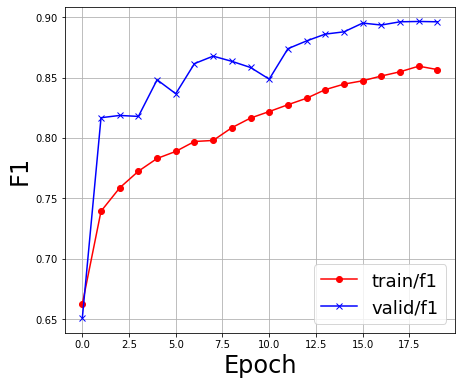
\includegraphics[width=0.5\textwidth]{f1.png}
    \caption{F1 Score by Epochs}
    \label{plot1}
\end{figure}

\begin{figure}[h!]
    \centering
    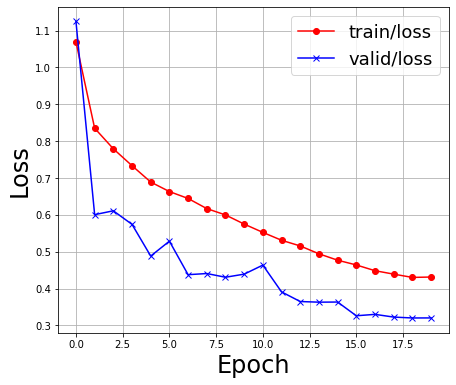
\includegraphics[width=0.5\textwidth]{loss.png}
    \caption{Loss by Epochs}
    \label{plot2}
\end{figure}

\begin{figure}[h!]
    \centering
    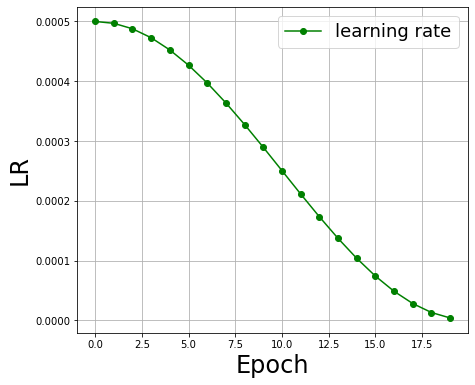
\includegraphics[width=0.5\textwidth]{lr.png}
    \caption{Learning Rate by Epochs}
    \label{plot3}
\end{figure}

These graphs represent the results obtained through the training of PyTorch Lightning:

\begin{itemize}
    \item F1 Score: This graph shows the evolution of the F1 score during the training process. The F1 score is a metric that combines both precision and recall into a single value, providing an overall measure of the model's performance. A higher F1 score indicates that the model is better at correctly predicting both positive and negative samples. In the graph, the y-axis represents the F1 score, and the x-axis represents the training epochs. Ideally, the F1 score should increase as the model is trained, indicating that it is becoming more accurate.
          We can see here that this is the case for both the training and validation set. There are however several moments of loss of accuracy that we cannot explain.
    \item Loss: This graph shows the evolution of the loss function during the training process. The loss function measures the discrepancy between the predicted and actual outputs of the model. In the graph, the y-axis represents the value of the loss function, and the x-axis represents the training epochs. The goal of training a machine learning model is to minimize the loss function, so the loss graph should show a decreasing trend over time. A decreasing trend indicates that the model is learning and becoming better at making predictions.
          As expected given the previous graph, both sets tend to lose loss over the epochs, and there are still several spikes of regaining loss for the validation set as witnessed earlier.
    \item Learning Rate: This graph shows the evolution of the learning rate during the training process. The learning rate determines the step size at which the model parameters are updated during training. In the graph, the y-axis represents the learning rate, and the x-axis represents the training epochs. The learning rate is typically adjusted during training to optimize the performance of the model. The learning rate graph can help identify potential issues with the training process, such as a learning rate that is too high or too low, which can result in the model not converging to a good solution.
          Here our learning rate slowly but surely converges towards zero, and the training stops before he has the occasion of drifting away from it, as would have happened had it not be stopped there.
\end{itemize}

\section{Best Practices and Tips for Using PyTorch Lightning}

\subsection{Code Organization}

\subsubsection{Overview}

Effective code organization is essential for the development, maintenance, and collaboration of deep learning projects. A well-structured codebase enhances readability, reusability, and scalability, making it easier for developers to navigate, debug, and iterate on their models.

\subsubsection{PyTorch Lightning in Code Organization}

PyTorch Lightning's modular design and high-level API promote clean and well-organized code, resulting in improved code quality and maintainability. Key aspects of code organization in PyTorch Lightning include:

\begin{itemize}
    \item LightningModule: PyTorch Lightning's LightningModule enforces a clean organization of model architecture, loss functions, and optimization logic, making it easier to understand, reuse, and share individual components of a deep learning project.
    \item LightningDataModule: The LightningDataModule component encourages the separation of data processing logic from the model architecture, promoting a more organized and modular codebase. This separation allows developers to reuse and share data processing logic across different models and tasks.
    \item Trainer: The Trainer component in PyTorch Lightning abstracts away the training loop and provides a standardized interface for configuring and launching the training process. This abstraction reduces boilerplate code and helps maintain a consistent structure across different projects.
    \item Callbacks and Loggers: PyTorch Lightning's built-in callbacks and loggers enable the extension and customization of the training process without cluttering the core components of the codebase. This separation ensures that the training logic remains focused and easier to understand.
    \item Integration with PyTorch Ecosystem: PyTorch Lightning's compatibility with the PyTorch ecosystem allows developers to leverage existing libraries and tools, reducing the need to reinvent the wheel and ensuring a consistent code organization across projects.
\end{itemize}

\subsection{Hyperparameter Tuning}

\subsubsection{Overview}

Hyperparameter tuning is the process of optimizing the parameters of a machine learning model that are not learned during training. These parameters, such as learning rate, batch size, and network architecture, can significantly impact the performance of the model. Efficient hyperparameter tuning is crucial for achieving optimal model performance and avoiding overfitting or underfitting.

\subsubsection{PyTorch Lightning in Hyperparameter Tuning}

PyTorch Lightning facilitates hyperparameter tuning by offering a modular design, integration with popular optimization libraries, and built-in support for logging and visualization. Key aspects of hyperparameter tuning in PyTorch Lightning include:

\begin{itemize}
    \item Separation of Concerns: The modular design of PyTorch Lightning, encompassing LightningModule and LightningDataModule, encourages a clean separation of model architecture, loss functions, optimization logic, and data processing. This separation simplifies the process of adjusting hyperparameters and evaluating their effects on the model.
    \item Integration with Optimization Libraries: PyTorch Lightning is compatible with popular hyperparameter optimization libraries, such as Optuna, Ray Tune, and Hyperopt. This compatibility allows users to leverage advanced optimization techniques, like Bayesian optimization and random search, to find the optimal set of hyperparameters for their models.
    \item Trainer Configuration: The Trainer component in PyTorch Lightning offers a standardized interface for configuring and launching the training process. By adjusting the Trainer's arguments, users can easily experiment with different hyperparameters, such as learning rate schedules, batch sizes, and gradient accumulation steps.
    \item Callbacks and Loggers: PyTorch Lightning's built-in callbacks and loggers enable users to track, visualize, and evaluate the effects of different hyperparameters on model performance during training. This tracking helps users identify the optimal hyperparameter configurations for their specific tasks.
    \item Reproducibility: PyTorch Lightning provides built-in support for ensuring reproducibility across multiple training runs. By setting random seeds and configuring the Trainer, users can guarantee consistent results, which is essential for reliable hyperparameter tuning.
\end{itemize}

\subsection{Experiment Tracking}

\subsubsection{Overview}

Experiment tracking is an essential aspect of deep learning projects, as it helps developers monitor, compare, and analyze different models, hyperparameters, and training configurations. Effective experiment tracking enables researchers to identify the most promising approaches, iterate on their models, and share their findings with collaborators.

\subsubsection{PyTorch Lightning in Experiment Tracking}

PyTorch Lightning simplifies experiment tracking by offering built-in loggers, integration with popular logging and visualization platforms, and a modular design that promotes clean, organized code. Key aspects of experiment tracking in PyTorch Lightning include:

\begin{itemize}
    \item Built-in Loggers: PyTorch Lightning comes with built-in loggers for popular experiment tracking platforms such as TensorBoard, Weights \& Biases, Neptune, and Comet.ml. These loggers enable users to track, visualize, and analyze various aspects of their experiments, such as loss curves, evaluation metrics, and hyperparameters.
    \item Custom Loggers: PyTorch Lightning allows users to create custom loggers, enabling seamless integration with other logging platforms or in-house tools. Custom loggers offer users the flexibility to adapt the logging process to their specific requirements and preferences.
    \item Callbacks: The callback system in PyTorch Lightning allows users to extend and customize the training process, enabling the tracking of custom metrics, model checkpoints, and other experiment-related information. Callbacks help users monitor various aspects of their experiments and make informed decisions about model improvements.
    \item Modular Design: PyTorch Lightning's modular design, including LightningModule, LightningDataModule, and Trainer components, encourages clean and organized code. This organization simplifies the process of tracking and comparing different models, data processing techniques, and training configurations.
    \item Reproducibility: PyTorch Lightning provides built-in support for ensuring reproducibility across multiple training runs. By setting random seeds and configuring the Trainer, users can achieve consistent results, which is crucial for reliable experiment tracking and comparison.
\end{itemize}

\subsection{Debugging and Testing}

\subsubsection{Overview}

Debugging and testing are critical aspects of deep learning projects, ensuring the correctness, robustness, and reliability of models and their associated code. Effective debugging and testing practices help developers identify and fix errors, validate model performance, and ensure that the codebase remains maintainable and free of technical debt.

\subsubsection{PyTorch Lightning in Debugging and Testing}

PyTorch Lightning simplifies debugging and testing by offering a high-level API, a modular design, built-in testing utilities, and integration with popular debugging and testing tools. Key aspects of debugging and testing in PyTorch Lightning include:

\begin{itemize}
    \item Modular Design: PyTorch Lightning's modular design, including LightningModule and LightningDataModule, promotes clean and organized code, making it easier to identify, isolate, and fix errors in the model architecture, loss functions, optimization logic, and data processing.
    \item Built-in Testing Utilities: PyTorch Lightning provides built-in testing utilities, such as trainer.test(), which simplify the process of evaluating model performance on test datasets. Users can also define custom validation and test loops, enabling the use of application-specific testing and evaluation strategies.
    \item Debugging Mode: The Trainer component in PyTorch Lightning offers a debugging mode (fast\_dev\_run) that enables users to quickly verify that their code runs without errors. This mode accelerates the debugging process by executing a single training, validation, and test batch, allowing users to identify and fix issues before running full-scale training.
    \item Integration with Debugging and Testing Tools: PyTorch Lightning is compatible with popular Python debugging and testing tools, such as pdb, PySnooper, and pytest. This compatibility allows users to leverage familiar tools and techniques for identifying and fixing errors, validating model performance, and ensuring the overall quality of their codebase.
    \item Callbacks and Loggers: PyTorch Lightning's built-in callbacks and loggers enable users to track, visualize, and analyze various aspects of their experiments, helping them identify potential issues, such as overfitting, underfitting, or other anomalies in model performance.
\end{itemize}

\section{Limitations and Criticisms}

\subsection{Performance Overhead}

\subsubsection{Overview}

Performance overhead refers to the additional computational cost introduced by using a particular framework or library compared to a more basic or custom implementation. In deep learning, minimizing performance overhead is essential for efficient training and inference, especially when working with large-scale datasets and complex models.

\subsubsection{PyTorch Lightning in Performance Overhead}

PyTorch Lightning aims to minimize performance overhead while providing users with a high-level API, modular design, and various utilities for training deep learning models. Key aspects of performance overhead in PyTorch Lightning include:

\begin{itemize}
    \item Lightweight Wrapper: PyTorch Lightning is designed as a lightweight wrapper around PyTorch, focusing on providing a user-friendly interface and advanced features while minimizing additional computational cost. Most of the operations in PyTorch Lightning are implemented using native PyTorch functions, ensuring optimal performance.
    \item Distributed Training: PyTorch Lightning's Trainer component offers built-in support for distributed training across multiple GPUs, TPUs, and clusters. This support enables users to efficiently scale their models for large-scale problems and complex environments, reducing the overall training time and associated costs.
    \item Customizability: The flexibility of PyTorch Lightning allows users to create custom layers, models, and training loops, enabling them to optimize their implementations for specific tasks and performance requirements. This customizability helps users minimize performance overhead by tailoring their code to their specific needs.
    \item Profiling and Optimization: PyTorch Lightning integrates with popular profiling tools, such as PyTorch's built-in profiler and NVIDIA's Nsight tools, enabling users to identify performance bottlenecks and optimize their code accordingly. By addressing these bottlenecks, users can minimize performance overhead and improve the efficiency of their models.
    \item Ongoing Development: The PyTorch Lightning development team actively works on improving the framework's performance and reducing overhead. As a result, new releases often include optimizations and enhancements that further minimize the performance impact of using PyTorch Lightning.
\end{itemize}

\subsection{Learning Curve}

\subsubsection{Overview}

The learning curve refers to the time and effort required for users to become proficient with a new framework, library, or tool. In deep learning, a gentle learning curve is crucial for enabling developers to quickly adopt new technologies and apply them to their specific tasks and projects.

\subsubsection{PyTorch Lightning in Learning Curve}

PyTorch Lightning offers a user-friendly API, extensive documentation, and a strong community, which together contribute to a gentle learning curve for developers. Key aspects of the learning curve in PyTorch Lightning include:

\begin{itemize}
    \item Familiarity with PyTorch: As a high-level wrapper around PyTorch, PyTorch Lightning builds upon the familiar PyTorch API, making it easier for developers with PyTorch experience to transition to using PyTorch Lightning.
    \item Intuitive API: PyTorch Lightning's API is designed to be intuitive and straightforward, abstracting away boilerplate code and focusing on the essential components of deep learning projects, such as model architecture, loss functions, and data processing.
    \item Modular Design: The modular design of PyTorch Lightning, including LightningModule, LightningDataModule, and Trainer components, promotes a clear separation of concerns, making it easier for users to understand, organize, and maintain their code.
    \item Extensive Documentation: PyTorch Lightning provides comprehensive documentation, including guides, tutorials, and API reference materials, which help users quickly learn and adopt the framework. The documentation covers a wide range of topics, from basic usage to advanced features, catering to users with varying levels of expertise.
    \item Active Community: PyTorch Lightning boasts a vibrant and supportive community, which contributes to the framework's development, provides support through forums and chat channels, and shares resources, such as blog posts, research papers, and code examples.
    \item Integration with Existing Tools: PyTorch Lightning's compatibility with popular deep learning libraries, experiment tracking platforms, and optimization tools allows users to leverage their existing knowledge and resources, further reducing the learning curve.
\end{itemize}

\subsection{Compatibility Issues}

\subsubsection{Overview}

Compatibility issues refer to the challenges faced when integrating a new framework, library, or tool with existing code, infrastructure, or workflows. In deep learning, minimizing compatibility issues is crucial for seamless adoption of new technologies and maximizing the benefits of existing tools and resources.

\subsubsection{PyTorch Lightning in Compatibility Issues}

PyTorch Lightning is designed to be compatible with a wide range of tools and libraries, minimizing the compatibility issues users may face when adopting the framework. Key aspects of compatibility in PyTorch Lightning include:

\begin{itemize}
    \item PyTorch Ecosystem: As a high-level wrapper around PyTorch, PyTorch Lightning is inherently compatible with the PyTorch ecosystem, allowing users to leverage existing PyTorch libraries, pre-trained models, and code snippets without major modifications.
    \item Integration with Popular Tools: PyTorch Lightning offers built-in integration with popular deep learning libraries, experiment tracking platforms, optimization tools, and visualization frameworks. This integration allows users to seamlessly incorporate PyTorch Lightning into their existing workflows and toolchains.
    \item Customizability: The flexibility of PyTorch Lightning enables users to create custom layers, models, training loops, callbacks, and loggers, facilitating seamless integration with in-house tools and frameworks, as well as other third-party libraries.
    \item Cross-framework Compatibility: While PyTorch Lightning is primarily designed for use with PyTorch, it is also compatible with other deep learning frameworks, such as TensorFlow and Keras, through the use of PyTorch's ONNX support for model conversion and interoperability.
    \item Python Version Compatibility: PyTorch Lightning supports a range of Python versions, ensuring compatibility with various Python environments and minimizing the need for users to upgrade or downgrade their Python installations.
    \item Continuous Development: The PyTorch Lightning development team actively works on improving compatibility with existing tools and libraries, as well as addressing any compatibility issues reported by the user community. As a result, new releases often include enhancements and bug fixes that further reduce compatibility issues.
\end{itemize}

\section{Future Developments and Trends}

\subsection{New Features and Improvements}

\subsubsection{Overview}

As an actively developed framework, PyTorch Lightning continually introduces new features and improvements to enhance its capabilities and address the evolving needs of the deep learning community. This section highlights some of the recent and upcoming features and improvements in PyTorch Lightning.

\subsubsection{New Features and Improvements in PyTorch Lightning}

\begin{itemize}
    \item Enhanced Distributed Training: PyTorch Lightning is continuously improving its support for distributed training across multiple GPUs, TPUs, and clusters, making it easier for users to scale their models and efficiently train large-scale deep learning systems.
    \item Improved Profiling and Optimization: PyTorch Lightning is working on integrating more advanced profiling tools and optimization techniques, enabling users to better understand the performance characteristics of their models and optimize their code for maximum efficiency.
    \item Expanded Library Integration: The framework actively seeks to integrate with more third-party libraries and tools, expanding its compatibility and providing users with a broader ecosystem of resources to support their deep learning projects.
    \item Advanced Callbacks and Loggers: PyTorch Lightning aims to introduce new built-in callbacks and loggers for popular experiment tracking platforms and visualization tools, making it even more convenient for users to track, analyze, and share their experiments.
    \item Improved Hyperparameter Tuning: The framework is working on enhancing its support for hyperparameter tuning, including integration with more optimization libraries and the development of new strategies for efficient and effective hyperparameter optimization.
    \item Enhanced Model Deployment: PyTorch Lightning is actively working on simplifying the deployment of trained models to various platforms, such as cloud services, edge devices, and web applications, making it easier for users to bring their models to production environments.
    \item Additional Pre-built Models and Architectures: The framework plans to include more pre-built models and architectures for various domains, such as computer vision, natural language processing, and reinforcement learning, making it even more convenient for users to adopt state-of-the-art techniques in their projects.
    \item Community-driven Development: PyTorch Lightning actively encourages community involvement in the development process, incorporating user feedback and suggestions to prioritize new features and improvements that address the needs of the deep learning community.
\end{itemize}

\subsection{Integration with other frameworks and tools}

\subsubsection{Overview}

The ability to integrate with various frameworks and tools is critical for any deep learning framework, as it allows users to leverage a diverse range of resources and techniques in their projects. PyTorch Lightning is designed to be compatible with many popular deep learning libraries, experiment tracking platforms, and optimization tools, simplifying integration and offering users a rich ecosystem of tools and resources.

\subsubsection{Integration with other frameworks and tools in PyTorch Lightning}

\begin{itemize}
    \item Deep Learning Libraries: PyTorch Lightning is compatible with numerous deep learning libraries built on top of PyTorch, such as torchvision, torchtext, and torchaudio. This compatibility allows users to easily incorporate advanced techniques, architectures, and pre-trained models from these libraries into their projects.
    \item Experiment Tracking Platforms: PyTorch Lightning provides built-in loggers for popular experiment tracking platforms, such as TensorBoard, Weights \& Biases, Neptune, and Comet.ml, enabling users to monitor, compare, and analyze their experiments with minimal additional setup.
    \item Optimization Tools: The framework is compatible with various optimization libraries, such as Optuna and Ray Tune, which can be used for hyperparameter tuning and model optimization, further improving the efficiency and performance of deep learning projects.
    \item Visualization Tools: PyTorch Lightning integrates with popular visualization tools, such as Matplotlib, Plotly, and Seaborn, allowing users to create custom visualizations of their data, model architectures, and experiment results.
    \item Distributed Training: PyTorch Lightning supports distributed training across multiple GPUs, TPUs, and clusters using popular distributed computing libraries, such as Horovod and DeepSpeed, enabling users to scale their models and efficiently train large-scale systems.
    \item Deployment Platforms: The framework is compatible with various model deployment platforms, such as ONNX Runtime, TensorFlow Serving, and NVIDIA Triton Inference Server, simplifying the process of deploying trained models to various environments, including cloud services, edge devices, and web applications.
    \item Other Deep Learning Frameworks: Although primarily designed for use with PyTorch, PyTorch Lightning can be used alongside other deep learning frameworks, such as TensorFlow and Keras, through the use of PyTorch's ONNX support for model conversion and interoperability.
    \item Python Ecosystem: PyTorch Lightning is built on top of the Python programming language, making it inherently compatible with the vast ecosystem of Python libraries and tools, such as NumPy, SciPy, and Pandas, which can be used for data manipulation, analysis, and visualization.
\end{itemize}

\subsection{Community Growth and Involvement}

\subsubsection{Overview}

A strong and active community is essential for the growth and success of any deep learning framework, as it drives innovation, offers support, and contributes to the development of new features and improvements. PyTorch Lightning has built a vibrant and supportive community, which plays a significant role in shaping the framework and addressing the evolving needs of the deep learning community.

\subsubsection{Community Growth and Involvement in PyTorch Lightning}

\begin{itemize}
    \item Open Source Contributions: As an open-source project, PyTorch Lightning actively encourages contributions from the community, including bug fixes, new features, and improvements to the codebase. This collaborative development model allows the framework to rapidly evolve and adapt to the needs of the deep learning community.
    \item Support and Knowledge Sharing: The PyTorch Lightning community offers support through various channels, such as forums, chat platforms, and social media. Users can ask questions, share their experiences, and learn from one another, fostering a collaborative and supportive environment.
    \item Tutorials and Workshops: Members of the community often create and share tutorials, workshops, and webinars, covering various aspects of PyTorch Lightning, from basic usage to advanced features. These resources help users quickly learn and adopt the framework, lowering the learning curve and accelerating their projects.
    \item Research and Publications: The PyTorch Lightning community is actively involved in cutting-edge research, using the framework to develop novel deep learning techniques and architectures. Researchers often share their findings in the form of research papers, blog posts, and presentations, contributing to the advancement of the field.
    \item Code Examples and Project Showcases: Community members contribute by sharing code examples, best practices, and showcasing their projects built using PyTorch Lightning. These examples serve as inspiration and learning resources for other users and help demonstrate the capabilities of the framework.
    \item Networking and Collaboration: The PyTorch Lightning community offers opportunities for networking and collaboration among users, researchers, and developers. This collaboration fosters the exchange of ideas and expertise, driving innovation and the development of new techniques and applications.
    \item Feedback and Feature Requests: The community plays an essential role in shaping the future of PyTorch Lightning by providing feedback, reporting issues, and suggesting new features and improvements. The development team actively incorporates this feedback to prioritize enhancements that address the needs of the deep learning community.
\end{itemize}

\section{Conclusion}

\subsection{Summary of Key Points}

\subsubsection{Overview}

This section provides a summary of the key points discussed in the report, highlighting the main aspects of PyTorch Lightning, its features, comparisons with other frameworks, and the role of the community.

\subsubsection{Summary of Key Points}

\begin{itemize}
    \item PyTorch Lightning is a high-level wrapper around PyTorch that simplifies the development of deep learning models, removing boilerplate code and providing a more organized, flexible, and scalable structure.
    \item The framework is built around three main components: LightningModule, LightningDataModule, and Trainer, which promote a clear separation of concerns and facilitate code organization, readability, and reusability.
    \item PyTorch Lightning offers various advanced features, such as distributed training, automatic mixed-precision training, and built-in callbacks and loggers, which help streamline the development process and improve model performance.
    \item The framework has been compared with other popular deep learning frameworks, including TensorFlow, Keras, Fast.ai, and MXNet, based on criteria such as code organization, hyperparameter tuning, experiment tracking, debugging, and testing.
    \item PyTorch Lightning is suitable for a wide range of deep learning applications, such as computer vision, natural language processing, reinforcement learning, and generative models.
    \item The framework offers advantages in terms of code organization, hyperparameter tuning, experiment tracking, debugging, and testing, which can help improve productivity and accelerate deep learning projects.
    \item PyTorch Lightning has a gentle learning curve, thanks to its intuitive API, extensive documentation, and active community, making it easy for developers to quickly learn and adopt the framework.
    \item The framework is designed to minimize compatibility issues, supporting integration with a wide range of tools and libraries, such as deep learning libraries, experiment tracking platforms, optimization tools, visualization tools, and deployment platforms.
    \item PyTorch Lightning continuously introduces new features and improvements, ensuring that it remains at the forefront of deep learning frameworks and addressing the evolving needs of the deep learning community.
    \item The framework's integration with other frameworks and tools enables users to leverage a diverse range of resources and techniques in their projects, simplifying integration and offering a rich ecosystem of tools and resources.
    \item The PyTorch Lightning community plays a significant role in the growth and success of the framework, driving innovation, offering support, and contributing to the development of new features and improvements.
\end{itemize}

\subsection{Overall Assessment of PyTorch Lightning}

\subsubsection{Overview}

In this section, we provide an overall assessment of PyTorch Lightning, taking into account the key features, advantages, and limitations of the framework, as well as the role of the community in its development.

\subsubsection{Overall Assessment}

\begin{itemize}
    \item Strengths: PyTorch Lightning offers several advantages, including a simplified API, clear code organization, and advanced features such as distributed training, automatic mixed-precision training, and built-in callbacks and loggers. These strengths make PyTorch Lightning a powerful and flexible deep learning framework that caters to a wide range of applications and user needs.
    \item Compatibility: The framework's compatibility with various tools, libraries, and frameworks, as well as its support for multiple Python versions, ensures seamless integration with existing codebases and workflows, reducing potential barriers to adoption.
    \item Community: The active and supportive PyTorch Lightning community contributes to the development of the framework, provides resources and support, and plays a crucial role in driving innovation, making the framework more appealing to new and experienced users alike.
    \item Continuous Improvement: The ongoing development of new features and improvements ensures that PyTorch Lightning remains at the forefront of deep learning frameworks, offering users the latest advancements and techniques to optimize their projects.
    \item Learning Curve: The gentle learning curve, extensive documentation, and rich ecosystem of tutorials and examples make PyTorch Lightning accessible to developers with varying levels of experience, enabling them to quickly learn and adopt the framework for their deep learning projects.
    \item Limitations: While PyTorch Lightning offers many advantages, it may not be the best choice for all use cases. For instance, developers who are already experienced with another deep learning framework may face a learning curve when transitioning to PyTorch Lightning. Additionally, certain niche applications or specific requirements may not be fully supported by the framework, necessitating the use of custom extensions or alternative solutions.
\end{itemize}

In conclusion, PyTorch Lightning is a powerful, flexible, and user-friendly deep learning framework that simplifies model development and offers advanced features for a wide range of applications. Its strong community, continuous growth, and integration with other frameworks and tools make it an excellent choice for deep learning practitioners. While it may not be ideal for every use case, its numerous strengths and the support of an active community make PyTorch Lightning a compelling option for developers seeking to accelerate their deep learning projects and improve overall productivity.

\section{References}

\begin{itemize}
    \item Falk, W. (2021). PyTorch Lightning.
    \item PyTorch Lightning Documentation. (2021).
    \item Paszke, A., Gross, S., Massa, F., Lerer, A., Bradbury, J., Chanan, G., ... \& Desmaison, A. (2019). PyTorch: An imperative style, high-performance deep learning library. Advances in Neural Information Processing Systems, 32, 8026-8037.
    \item Abadi, M., Agarwal, A., Barham, P., Brevdo, E., Chen, Z., Citro, C., ... \& Ghemawat, S. (2016). TensorFlow: Large-scale machine learning on heterogeneous distributed systems. arXiv preprint arXiv:1603.04467.
    \item Chollet, F., et al. (2015). Keras.
    \item Howard, J., \& Gugger, S. (2020). Fastai: A layered API for deep learning. Information, 11(2), 108.
    \item Chen, T., Li, M., Li, Y., Lin, M., Wang, N., Wang, M., ... \& Zhang, Q. (2015). MXNet: A flexible and efficient machine learning library for heterogeneous distributed systems. arXiv preprint arXiv:1512.01274.
    \item Optuna: A Next-generation Hyperparameter Optimization Framework. (2021).
    \item Liaw, R., Liang, E., Nishihara, R., Moritz, P., Gonzalez, J. E., \& Stoica, I. (2018). Tune: A research platform for distributed model selection and training. arXiv preprint arXiv:1807.05118.
    \item ONNX Runtime: Cross-Platform, High-Performance ML Inferencing and Training. (2021).
\end{itemize}

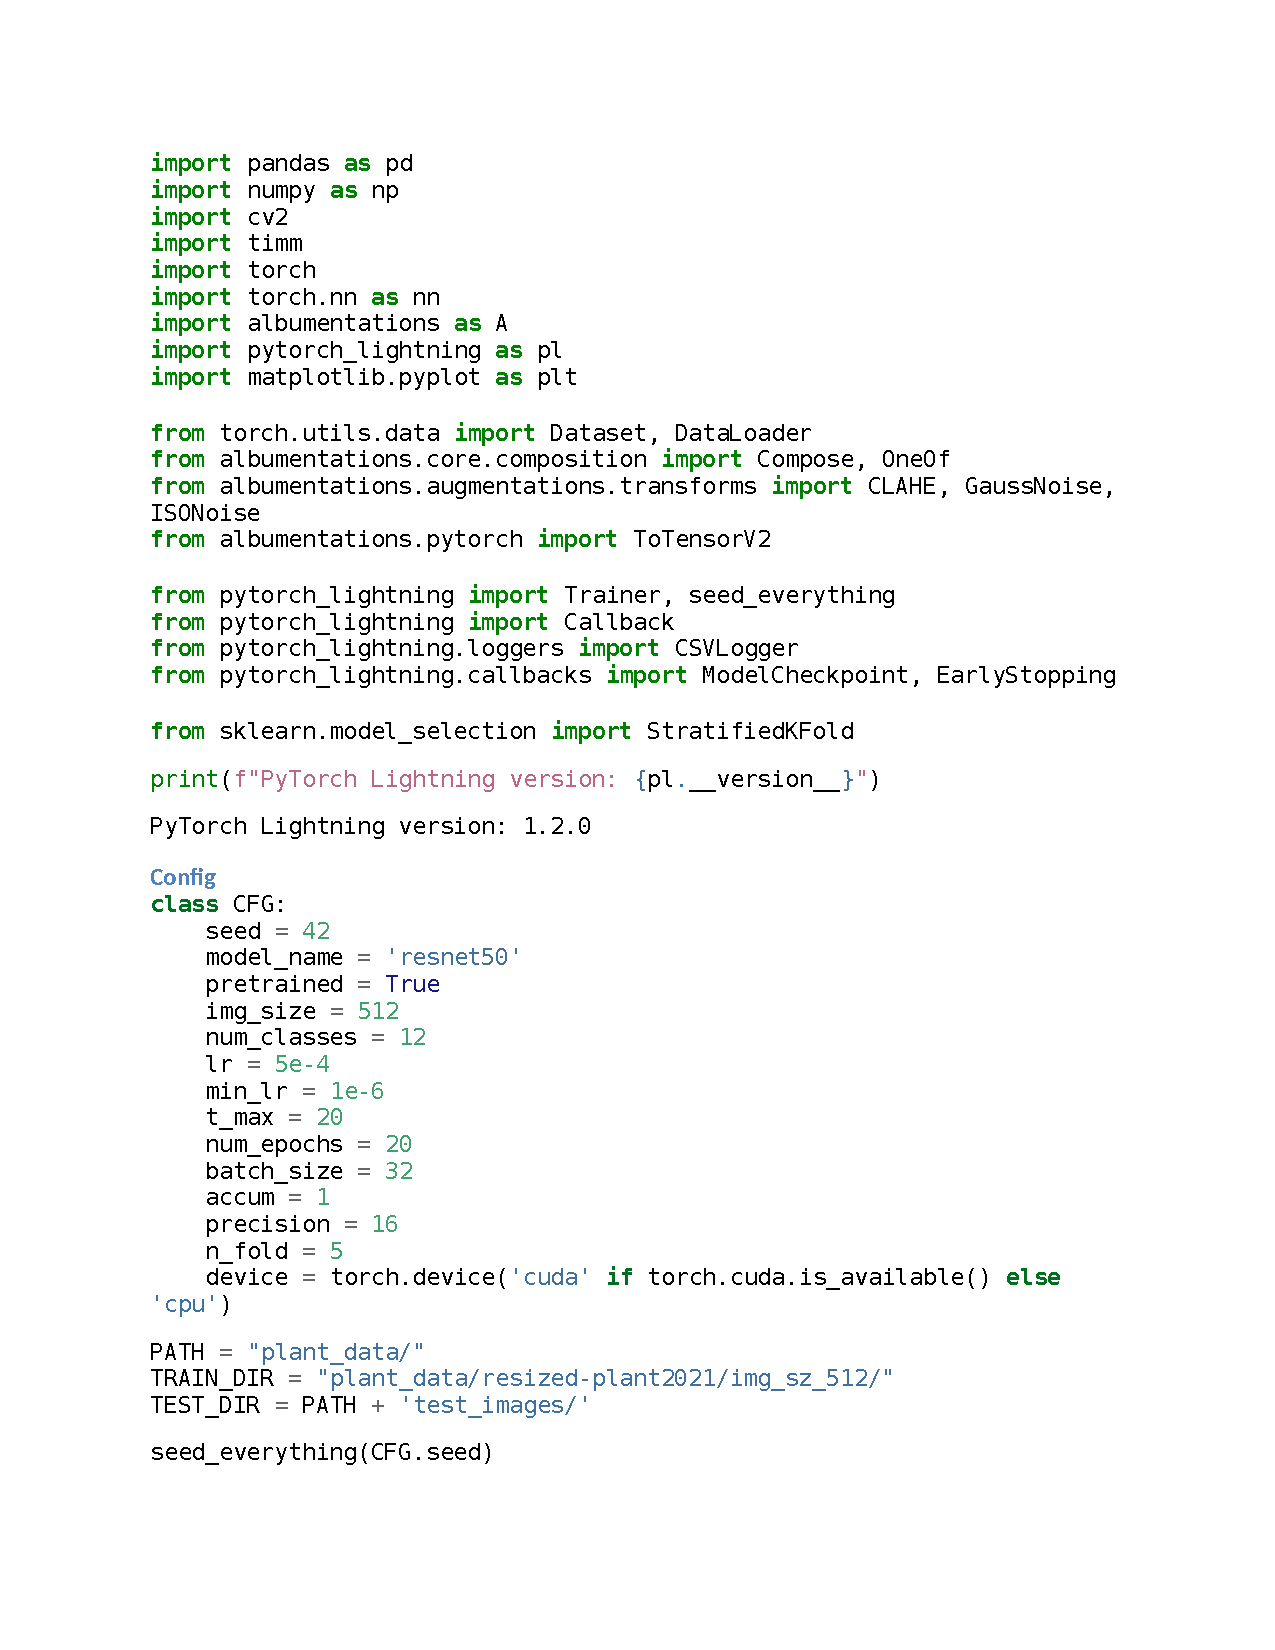
\includepdf[pages=-]{pytorch_plant.pdf}

\end{document}